\begin{frame}
    \frametitle{Béziérovy plochy}

    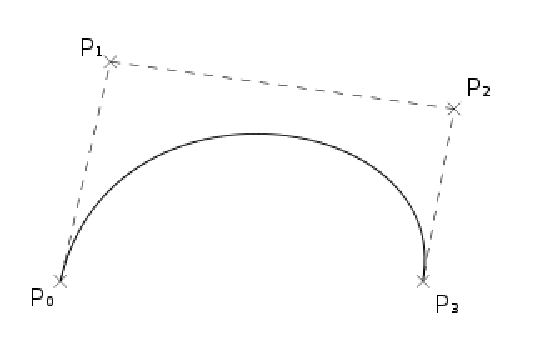
\includegraphics[height=.3\textheight]{pics/tessellationBezier/bezier.eps}

    \begin{eqnarray*}
        B_{n,k}(t) &=& {n\choose k}t^k\left(1-t\right)^{\left(n-k\right)}\\
        P(t)      &=& \left[\left(B_{n,0}(t),\ldots,B_{n,n}(t)\right)\left(
            \begin{array}{ccc}
                x_0 & y_0 & \ldots\\
                x_1 & y_1 & \ldots\\
                &\ldots&
            \end{array}\right)\right]\\
        P_{\{x,y,z\}}(u,v) &=& \left[\left(B_{n,0}(u),\ldots,B_{n,n}(u)\right)K_{\{x,y,z\}}\left(
            \begin{array}{c}B_{n,0}(v)\\\ldots\\B_{n,n}(v)\end{array}\right)\right]
    \end{eqnarray*}
\end{frame}

\begin{frame}
    \frametitle{Racionální béziérky}

    Kontrolní body mají i váhu :
    \begin{equation*}
        P(t) = \frac{ \sum_{i=0}^n B_{i,n}(t) \mathbf{P_i w_i} }{ \sum_{i=0}^n B_{i,n}(t) \mathbf{w_i} }
    \end{equation*}
    \pause\vfill
    \begin{itemize}
        \item Váha táhne plochu blíž k bodu.
        \item Kontrolní body s vahou jsou homogenní souøadnice.
        \item Jdou bez problémù i promítnout.
    \end{itemize}
\end{frame}    

\begin{frame}[fragile]
\frametitle{Vertex Shader}
	{\scriptsize
	\begin{minted}[frame=lines]{glsl}
#version 410

uniform mat4 mvp;

layout(location=0) in vec4 position;

void main()
{
    gl_Position = mvp*position;
}
	\end{minted}
	}
\end{frame}

\begin{frame}[fragile]
\frametitle{Fragment Shader}
	{\scriptsize
	\begin{minted}[frame=lines]{glsl}
#version 410

flat in vec4 color;

out vec4 output;

void main()
{
    output = color;
}
	\end{minted}
	}
\end{frame}

\begin{frame}[fragile]
\frametitle{Control Shader}
	{\scriptsize
	\begin{minted}[frame=lines]{glsl}
#version 410

layout(vertices=16) out;

void main()
{
    gl_out[gl_InvocationID].gl_Positiono
        = gl_in[gl_InvocationID].gl_Position;
    if(gl_InvocationID == 0)
    {
        gl_TessLevelInner[0] = 8;
        gl_TessLevelInner[1] = 8;
        gl_TessLevelOuter[0] = 64;
        gl_TessLevelOuter[1] = 64;
        gl_TessLevelOuter[2] = 64;
        gl_TessLevelOuter[3] = 64;
    }
}
	\end{minted}
	}
\end{frame}

\begin{frame}[fragile]
\frametitle{Evaluation Shader}
	{\scriptsize
	\begin{minted}[frame=lines]{glsl}
#version 410
layout(quads, equal_spacing, ccw) in;
flat out vec4 color;
vec4 bernstein(float t)
{
  return vec4((1-t)*(1-t)*(1-t),3*t*(1-t)*(1-t),3*t*t*(1-t), t*t*t);
}
void main()
{
  vec4 bu = bernstein(gl_TessCoord.x);
  vec4 bv = bernstein(gl_TessCoord.y);
  vec4 position = vec4(0,0,0,0);
  for(int y = 0; y < 4; ++y)
    for(int x = 0; x < 4; ++x)
      position += bu[x]*bv[y]*gl_in[4*y+x].gl_Position;
  gl_Position = position;
  color = vec4(gl_TessCoord.xy,0,1);
}
	\end{minted}
	}
\end{frame}

